\chapter{Ensayos y Resultados}\label{Chapter4}

% \section{Infraestructura para el Desarrollo}

\section{Pruebas unitarias}

En la presente sección del documento se muestran únicamente algunos ejemplos de
todas las pruebas unitarias realizadas. Estas muestras representan una fracción
de la totalidad de pruebas unitarias llevadas a hechas durante el desarrollo del
proyecto. Se optó por incluir estos casos de prueba como ejemplos representativos
para ilustrar el proceso de verificación, ya que contando con más de 20 módulos
cada uno con multiples configuraciones no se consideró útil enriquecedor agregar
todos los casos.

Es importante destacar que el conjunto completo de pruebas unitarias, así como
otros aspectos relacionados con el desarrollo y la implementación, están
disponibles de forma completa en los \textit{pipeline} de CI de GitHub del
proyecto. Este repositorio, al ser público, proporciona acceso a todos los
detalles relevantes del proceso de desarrollo, incluidas las pruebas unitarias
completas, las funcionales, las de integración a nivel sistema, los \textit{linter}
y otros aspectos relevantes del flujo de trabajo de desarrollo.

Por lo tanto, para una visión exhaustiva y detallada de las pruebas unitarias
y otros elementos del proyecto, se recomienda consultar el \textit{pipeline} de
GitHub correspondiente, donde se encuentran disponibles de manera más adecuada
para un análisis completo en el contexto de una tesis.

% todo: AGREGAR LINK!!!!!

\subsection{Replicador de bits}

  Se corrieron las pruebas unitarias del replicador de bits: 

  {\scriptsize\begin{verbatim}
    Seeding Python random module with 1709476252
    Found test test_sdi_bit_rep.test_sdi_bit_rep
    running test_sdi_bit_rep (1/1)
    test_sdi_bit_rep passed
    *******************************************************************************************
    ** TEST                               STATUS  SIM TIME (ns)  REAL TIME (s)  RATIO (ns/s) **
    *******************************************************************************************
    ** test_sdi_bit_rep.test_sdi_bit_rep   PASS         300.00           0.00     192723.42  **
    *******************************************************************************************
    ** TESTS=1 PASS=1 FAIL=0 SKIP=0                     300.00           0.03       9765.47  **
    *******************************************************************************************
  \end{verbatim}}

  La simulación del módulo bit\_rep se realizó con éxito, confirmando el correcto
  funcionamiento del diseño. Durante la simulación, se observó que el módulo
  replicaba los bits de los datos de entrada 11 veces, ver figura~\ref{fig:bit-re},
  generando una salida de 20 bits en cada ciclo de reloj.

  \begin{figure}[h]
    \centering
    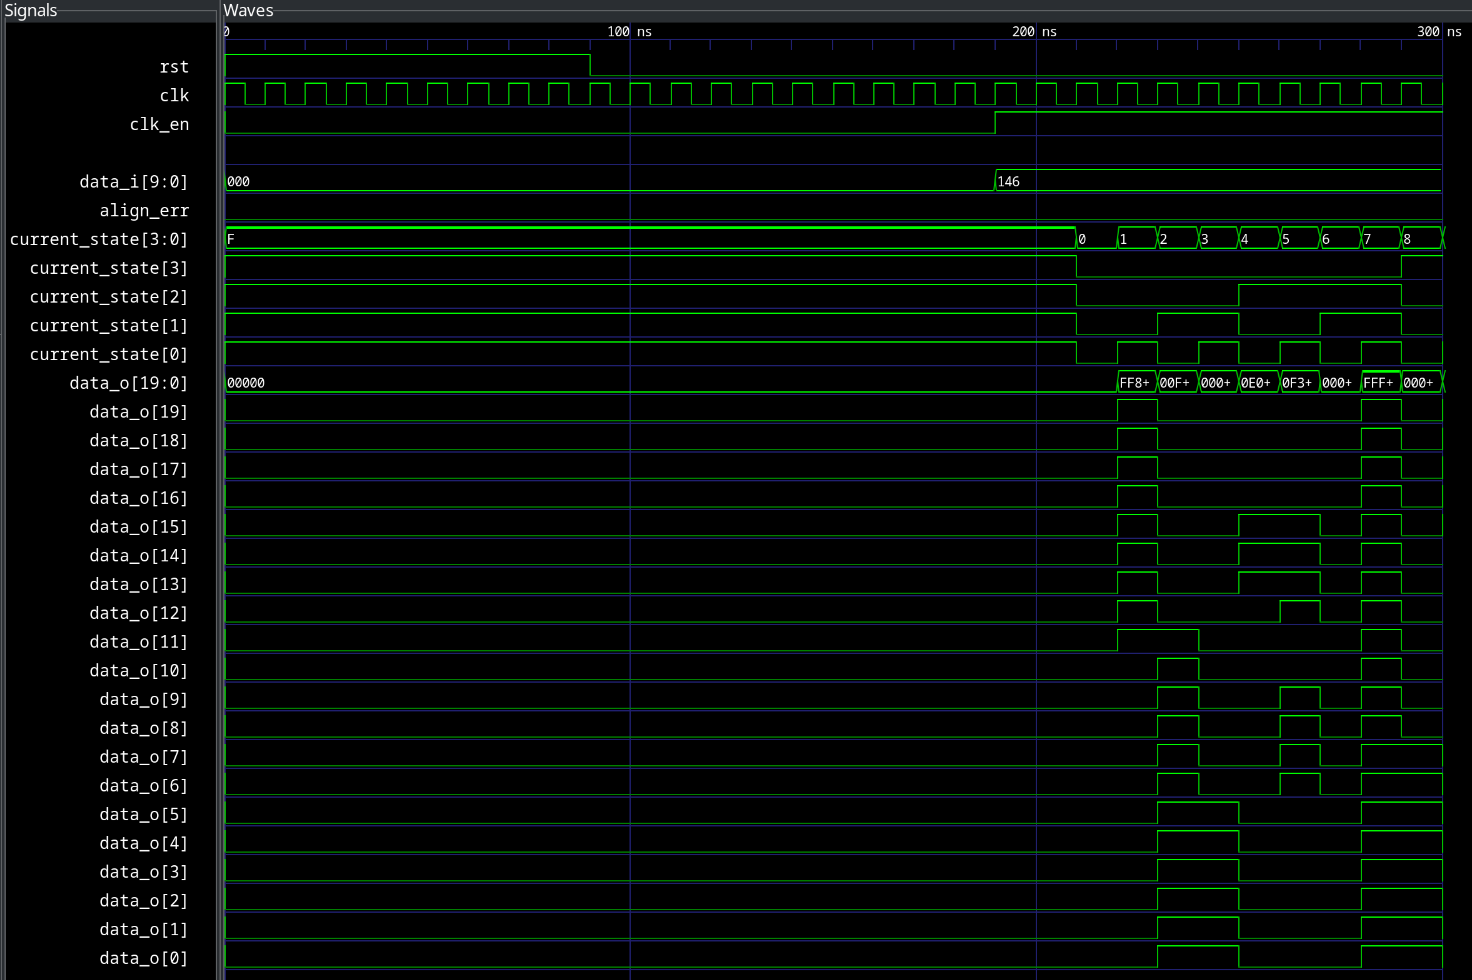
\includegraphics[width=1\textwidth]{./Figures/bit_rep.png}
    \caption{Simulación del módulo bit\_rep}\label{fig:bit-rep}
  \end{figure}
  
  Se verificó que la máquina de estados se alineaba automáticamente, garantizando
  un comportamiento adecuado independientemente de la cadencia inicial del reloj
  de habilitación. Además, no se detectaron desalineaciones en la cadencia 5/6/5/6
  durante la simulación. Estos resultados validan la funcionalidad esperada del
  módulo.

\subsection{Verificación de redundancia cíclica}

  Se corrieron las respectivas pruebas unitarias, tanto para el módulo capaz de
  calcular el CRC, como para los \textit{wrappers} que adaptan las señales del
  flujo transmisión y recepción de datos:

  {\scriptsize\begin{verbatim}
    Seeding Python random module with 1709474689
    Found test test_crc_insert.crc_insert_test
    running crc_insert_test (1/1)
    crc_insert_test passed
    *****************************************************************************************
    ** TEST                             STATUS  SIM TIME (ns)  REAL TIME (s)  RATIO (ns/s) **
    *****************************************************************************************
    ** test_crc_insert.crc_insert_test   PASS         430.36           0.00     244532.75  **
    *****************************************************************************************
    ** TESTS=1 PASS=1 FAIL=0 SKIP=0                   430.36           0.03      14103.80  **
    *****************************************************************************************
  \end{verbatim}}

  {\scriptsize\begin{verbatim}
    Seeding Python random module with 1709474535
    Found test test_crc_rx.crc_rx_test
    running crc_rx_test (1/1)
    test_crc_rx passed
    **************************************************************************************
    ** TEST                          STATUS  SIM TIME (ns)  REAL TIME (s)  RATIO (ns/s) **
    **************************************************************************************
    ** test_crc_rx.crc_rx_test        PASS         489.01           0.00     218972.36  **
    **************************************************************************************
    ** TESTS=1 PASS=1 FAIL=0 SKIP=0                489.01           0.03      17432.87  **
    **************************************************************************************
  \end{verbatim}}

  {\scriptsize\begin{verbatim}
    Seeding Python random module with 1709473164
    Found test test_crc18.crc18_test
    running crc18_test (1/1)
    crc18_test passed
    **************************************************************************************
    ** TEST                          STATUS  SIM TIME (ns)  REAL TIME (s)  RATIO (ns/s) **
    **************************************************************************************
    ** test_crc18.crc18_test          PASS         390.63           0.00     250945.16  **
    **************************************************************************************
    ** TESTS=1 PASS=1 FAIL=0 SKIP=0                390.63           0.03      11570.77  **
    **************************************************************************************
  \end{verbatim}}

  \begin{figure}[h]
    \centering
    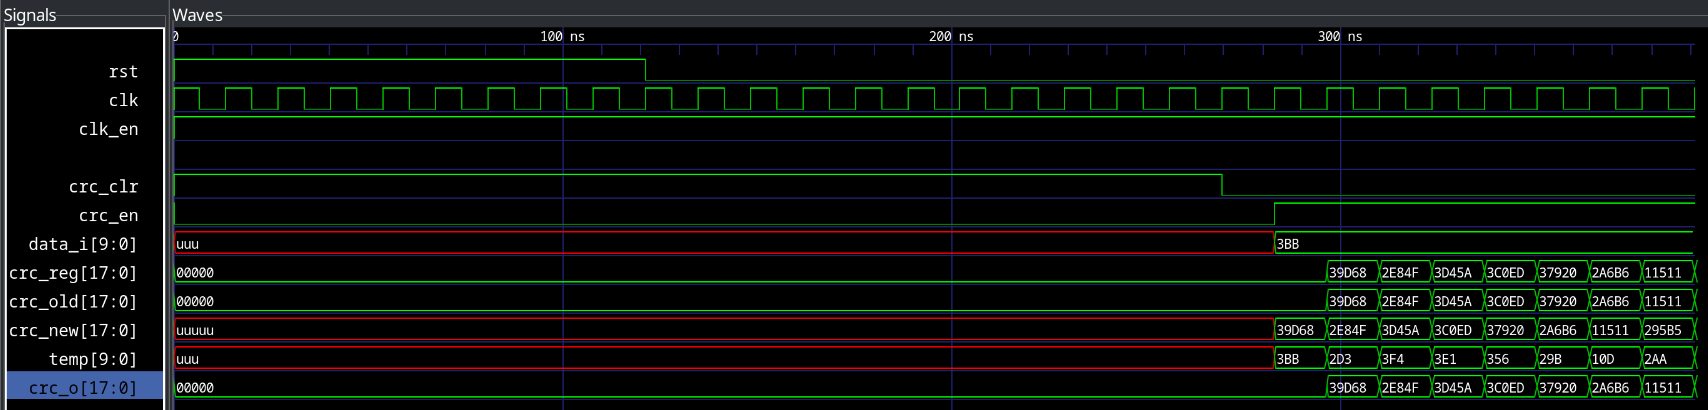
\includegraphics[width=1\textwidth]{./Figures/crc18.png}
    \caption{Simulación del módulo crc18}\label{fig:crc18}
  \end{figure}

  La simulación del módulo de verificación de redundancia cíclica se llevó a cabo
  con éxito, confirmando su correcto funcionamiento en la verificación del CRC,
  ver figuras \ref{fig:crc18} y \ref{fig:crc18-z}\@.
  Durante la simulación, se observó que el módulo calculaba correctamente el
  valor CRC para cada línea de video, tanto para los canales Y como para C.
  Además, se verificó que el valor CRC calculado se comparaba con el valor CRC
  recibido, activando la salida de error CRC correspondiente en caso de detectarse
  un error. Esta salida permaneció activada durante el tiempo de una línea de
  video, como se esperaba, hasta que se realizó la próxima verificación de CRC\@.

  \begin{figure}[h]
    \centering
    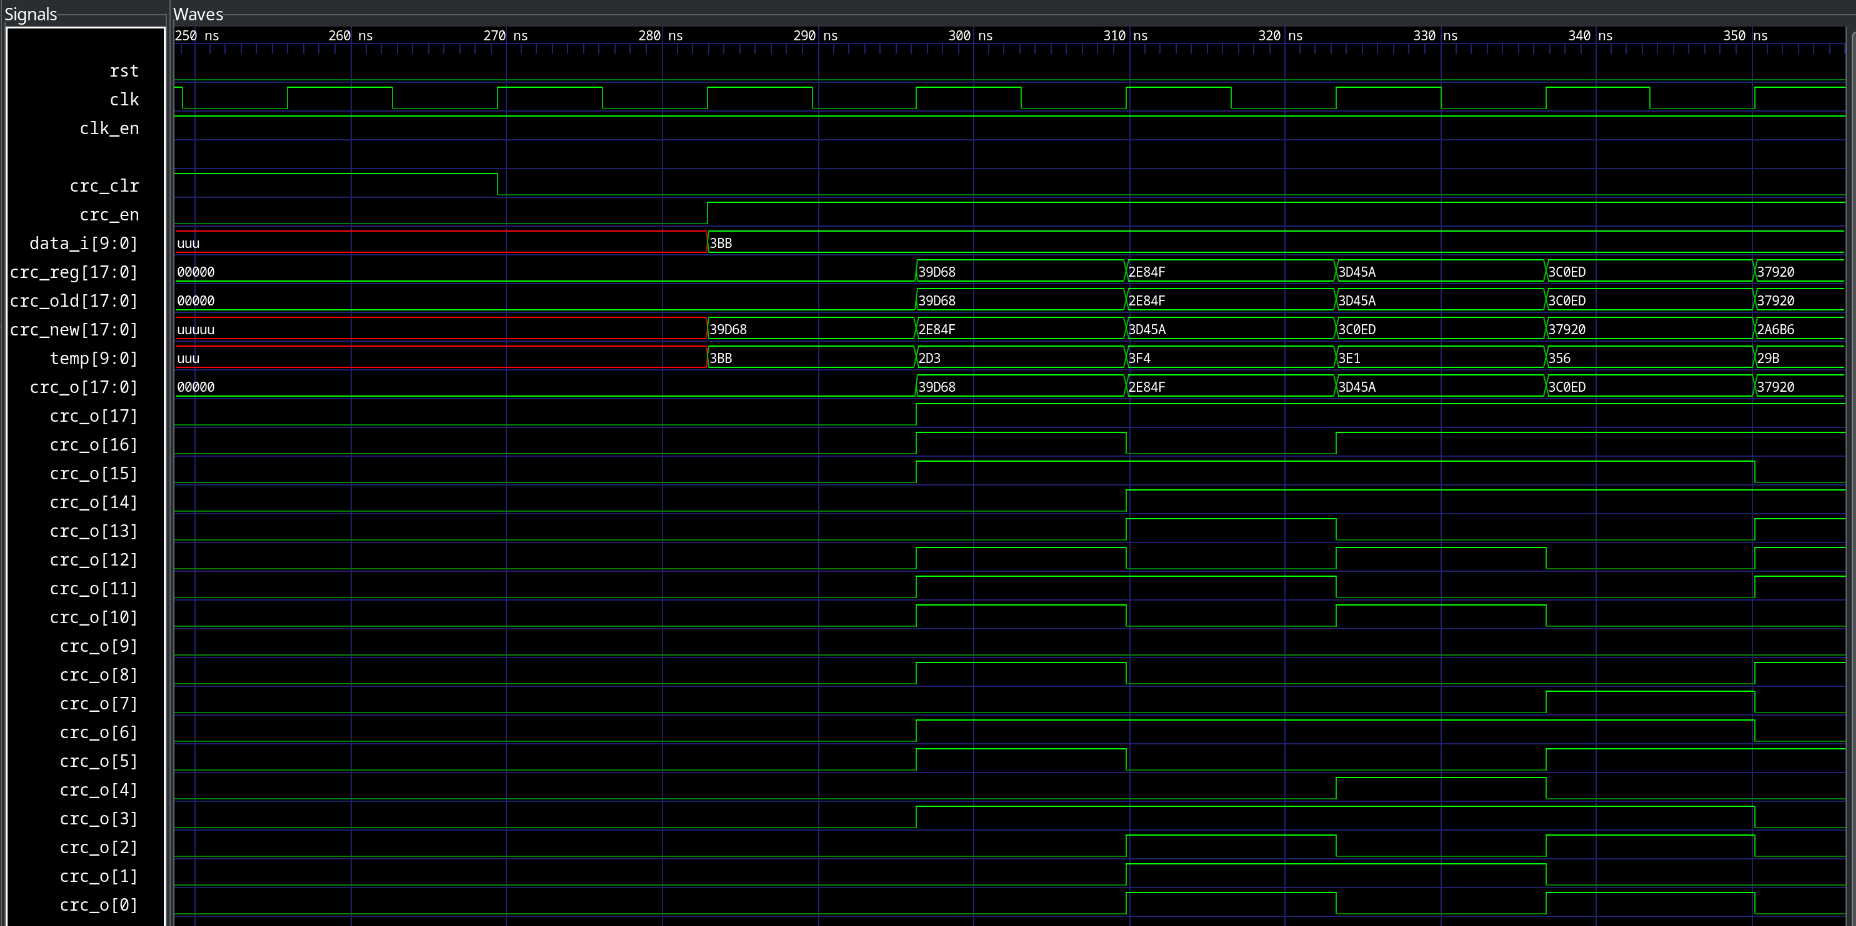
\includegraphics[width=1\textwidth]{./Figures/crc18_zoom.png}
    \caption{Simulación del módulo crc18 enfocada en los datos}\label{fig:crc18-z}
  \end{figure}

  Adicionalmente, se pudo observar que el módulo capturaba correctamente los
  valores del número de línea para ambos canales y los emitía adecuadamente.
  Estos valores del número de línea fueron válidos durante todo el tiempo de la
  línea, como se especificaba en la descripción del módulo.

\subsection{Codificador}

  {\scriptsize\begin{verbatim}
    Seeding Python random module with 1709472961
    Found test test_nrz_2_nrzi.nrzi_basic_test
    running nrzi_basic_test (1/1)
    [1, 0, 0, 1, 1, 0, 0, 1, 1]
    [1, 0, 0, 1, 1, 0, 0, 1, 1]
    nrzi_basic_test passed
    *****************************************************************************************
    ** TEST                             STATUS  SIM TIME (ns)  REAL TIME (s)  RATIO (ns/s) **
    *****************************************************************************************
    ** test_nrz_2_nrzi.nrzi_basic_test   PASS         296.34           0.00     249286.01  **
    *****************************************************************************************
    ** TESTS=1 PASS=1 FAIL=0 SKIP=0                   296.34           0.02      16257.78  **
    *****************************************************************************************
  \end{verbatim}}



{\scriptsize\begin{verbatim}
  
\end{verbatim}}

\section{Pruebas de integración}

\section{Simulación y Verificación}

La verificación y validación de código y modelos por medio de simulación es
un aspecto crucial para garantizar calidad y reducir tiempos de desarrollo,
sobre todo en sistemas críticos. La verificación garantiza con simulaciones y
permite la corrección del código, antes de hacer pruebas en el mundo real, que
son más lentas y costosas. La validación se relaciona con la conexión del
desarrollo con el mundo real y su uso previsto, implica contar con el
\textit{hardware} y el instrumental de medición. Además, en sistemas de alta
complejidad la simulación permite probar cada módulo por separado, técnica que
facilita la integración y permite distinguir con claridad los errores, lo que
acelera proceso de aprendizaje y comprensión del sistema. Por otro lado al ser
capaces de simular datos de cierto modelo, se garantiza que uno entiende el
modelo, sus restricciones y limitaciones.

% En este trabajo se llevaron a cabo test unitarios para cada módulo básico del
% desarrollo e incluso aquellos que integraban varios submódulos, usando GHDL,
% cocotb e integración continua en Github, pero para la verificación del sistema
% completo fue necesario usar Quartus y ModelSim, ya que no se contaba con los
% modelos de los Transceivers debido a que son herramientas propietarias.

\subsection{\textit{cocotb}}
\textit{cocotb} (por sus siglas en inglés \textit{COroutine based COsimulation
TestBench}) es un entorno de \textit{TestBench} de verificación de simulación
basado en corrutinas para verificar RTL (por sus siglas en inglés
\textit{Register Transfer Level}) descriptos en VHDL y SystemVerilog utilizando
Python.

Este \textit{Framework} es completamente gratuito, de código abierto (Licencia
BSD) y alojado en GitHub.\textit{cocotb} requiere un simulador para simular el
diseño HDL (por sus siglas en inglés \textit{Hardware Description Language}) y
se puede utilizar con una variedad de simuladores en multiples sistemas
operativos.

\textit{cocotb} fomenta la filosofía de reutilización de diseño y pruebas
aleatorias que UVM, sin embargo, está implementado en Python.

Con \textit{cocotb}, los HDL tradicionales se utilizan solo para el diseño en
sí, no para el banco de pruebas. Además, tiene soporte incorporado para
integrarse con sistemas de integración continua y fue diseñado específicamente
para reducir la sobrecarga de la creación de una prueba.También descubre
automáticamente las pruebas, por lo que no se requiere un paso adicional para
agregar una prueba a una regresión.

La verificación se realiza integramente con Python, lo cual tiene varias
ventajas por sobre el uso de SystemVerilog o VHDL para la verificación:

\begin{itemize}
  \item Es rápido escribir en Python, es un lenguaje muy productivo.
  \item Es fácil interfacear con otros lenguajes.
  \item Python tiene una enorme biblioteca de código existente para reutilizar.
  \item Python es interpretado: las pruebas se pueden editar y volver a ejecutar
  sin tener que recompilar el diseño.
  \item Python es popular: muchos más desarrolladores conocen Python que
  VHDL o SystemVerilog.
\end{itemize}

\subsection{Funcionamiento de \textit{cocotb}}

Un banco de pruebas típico de \textit{cocotb} no requiere código RTL adicional.
El Diseño Bajo Prueba (DUT, por sus siglas en inglés \textit{Design-Device
under Test}) se instancía como el \textit{toplevel} en el simulador sin ningún
código que haga de interfaz o \textit{wrapper}.\textit{cocotb} proporciona
estímulos a las entradas del DUT (o incluso más abajo en la jerarquía) y
supervisa las salidas directamente desde Python.

\begin{figure}[h]
  \centering
  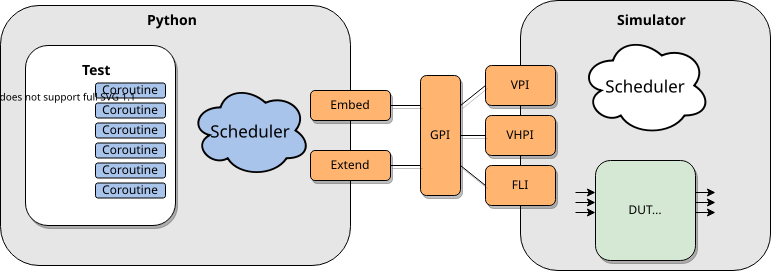
\includegraphics[width=0.7\textwidth]{./Figures/cocotb_overview.png}
  \caption{Visión general de \textit{cocotb}.}
\end{figure}

% Una prueba es simplemente una función Python. En cualquier momento, el simulador
% está avanzando en el tiempo o el código Python se está ejecutando. La palabra
% clave \texttt{await} se utiliza para indicar cuándo pasar el control de
% ejecución de vuelta al simulador. Una prueba puede generar múltiples corutinas,
% lo que permite flujos de ejecución independientes.

\subsection{Estructura Genérica de los \textit{Test} y sus resultados}

\section{Integración Continua}

La integración continua (CI, del inglés \textit{continuous integration}) es una
práctica que nace de la ingeniería de software, pero que en los últimos años se
a ido extendiendo a otras ramas de la ingeniería, que consiste en hacer
integraciones automáticas de un proyecto con cierta regularidad para así poder
detectar errores cuanto antes. Se entiende por integración la compilación o
síntesis y ejecución de pruebas de un proyecto completo y sus subsistemas. 

Por lo general se necesita un sistema de control de versiones que acompañe y
ejecute del proceso de CI\@. Los mismos también se complementan con otras
comprobaciones como las pruebas automatizadas de calidad del código, las
herramientas de revisión de estilo de sintaxis, entre otras.

Para pasar en limpio, los beneficios comúnmente citados de la integración
continua incluyen:
\begin{itemize}
  \item Detección temprana y mejorada de errores, y métricas que le permiten
  abordar los errores a tiempo, a veces tras solo unos minutos de la incorporación.
  \item Progreso continuo y demostrado para mejorar la retroalimentación.
  \item Mejor colaboración en equipo: todos los miembros del equipo pueden.
  cambiar el código, integrar el sistema y determinar rápidamente los conflictos
  con otras partes del del mismo.
  \item Integración mejorada del sistema, lo que reduce las sorpresas al final
  del ciclo de vida del desarrollo.
  \item Menos cambios paralelos para la fusión y prueba.
  \item Reducción de cantidad de errores durante las pruebas del sistema.
  \item Sistemas actualizados constantemente en los que realizar las pruebas.
\end{itemize}

En el caso de este trabajo se optó por usar Git como sistema de control de
versiones, más específicamente Github, que con Github Actions también entrega
la funcionalidad de integración continua.

% \section{Quartus y ModelSim}

\section{Resultados}

\subsection{Resultados Generales}

\subsection{Resultados por módulo}
